\begin{apendicesenv}

\partapendices

\chapter{\textit{Host-spot Cards}}

Nesse apêndice, serão apresentados os \textit{hot-spot cards} de cada \textit{hot-spot}, conforme apresentado por \cite{Fayad1999}.

\section{PathPlanner}

{\large \textbf{Nome do hot-spot:}} Algoritmo de Path Plannig

{\large \textbf{Graus de flexibilidade especificados:}}

\textbf{adaptação sem reinício:} sim

\textbf{adaptação pelo usuário final:} não

{\large \textbf{Descrição geral}}

Definição da trajetória em um mapa já conhecido a partir de um algoritmo estabelecido. Recebe o mapa com os obstáculos e espaços livres, o algoritmo a ser executado e os pontos iniciais e finais e retorna um grafo com os caminhos possíveis

{\large \textbf{Exemplo 1}}

Recebe-se o seguinte mapa, aonde a célula preta significa ocupado, branca significa livre e os pontos iniciais e finais marcados.

\begin{figure}[H]
	\centering
	\label{figXX}
		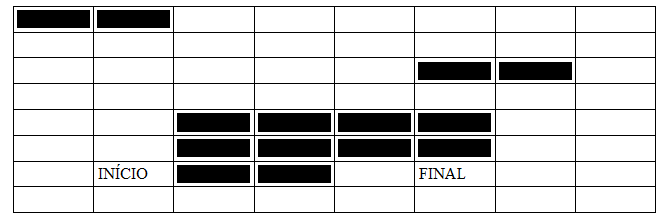
\includegraphics[keepaspectratio=true,scale=0.7]{figuras/mapahotspot1.PNG}
	\caption{mapa exemplo do \textit{hot-spot card} PathPlanner}
\end{figure}

Para o algorítimo Quadtree será gerado o grafo apresentado na Figura \label{figXX1}.

\begin{figure}[H]
	\centering
	\label{figXX1}
		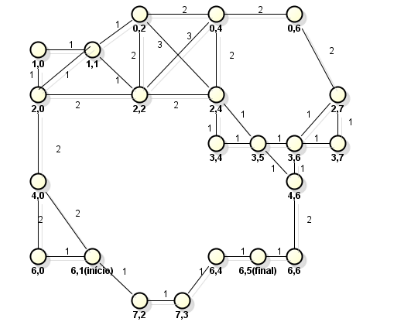
\includegraphics[keepaspectratio=true,scale=0.7]{figuras/grafohotspotcard1.PNG}
	\caption{resultado do exemplo 1 do \textit{hot-spot card} PathPlanner}
\end{figure}

{\large \textbf{Exemplo 2}}

Recebe-se o seguinte mapa, aonde a célula preta significa ocupado, branca significa livre e os pontos iniciais e finais marcados.

\begin{figure}[H]
	\centering
	\label{figXX2}
		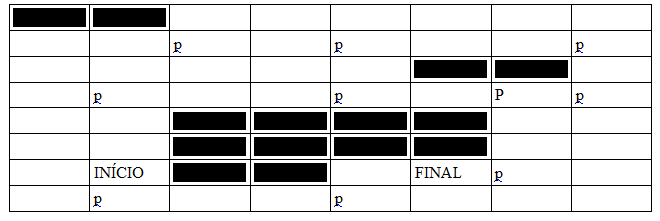
\includegraphics[keepaspectratio=true,scale=0.7]{figuras/mapahotspot2.PNG}
	\caption{mapa exemplo 2 do \textit{hot-spot card} PathPlanner}
\end{figure}

Para o algorítimo Grafo de Visibilidade gerará o grafo:

\begin{figure}[H]
	\centering
	\label{figXX3}
		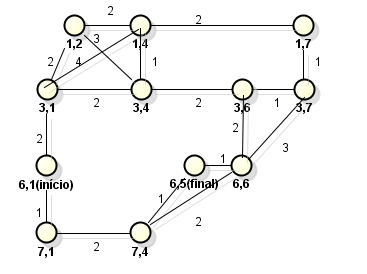
\includegraphics[keepaspectratio=true,scale=0.7]{figuras/grafohotspotcard2.PNG}
	\caption{resultado do exemplo 2 do \textit{hot-spot card} PathPlanner}
\end{figure}

\section{BestPath}

{\large \textbf{Nome do hot-spot:}} Algoritmo de Menor caminho

{\large \textbf{Graus de flexibilidade especificados:}}

\textbf{adaptação sem reinício:} sim

\textbf{adaptação pelo usuário final:} não

{\large \textbf{Descrição geral}}

Definição do menor caminho entre um nó e outro em um grafo, retornando a lista de nós com menor custo possível. O grafo e os nós de início e fim são recebidos via construtor e é retornada uma lista de nós.

{\large \textbf{Exemplo 1}}

Recebe-se o grafo abaixo, aonde o inicial é “6,1” e o final é “6,5”.

\begin{figure}[H]
	\centering
	\label{figXX}
		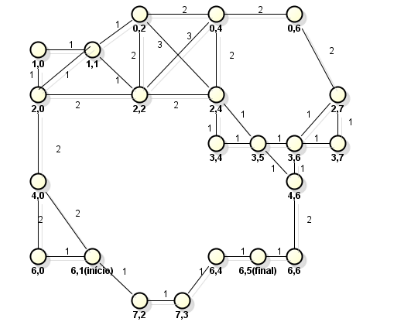
\includegraphics[keepaspectratio=true,scale=0.7]{figuras/grafohotspotcard1.PNG}
	\caption{grafo exemplo do \textit{hot-spot card} BestPath}
\end{figure}

Para o algorítimo Djikstra, será gerado o grafo: 6,1 -> 7,2 -> 7,3 -> 6,4 -> 6,5.

{\large \textbf{Exemplo 2}}

Recebe-se o grafo abaixo, aonde o inicial é “6,1” e o final é “6,5”.

\begin{figure}[H]
	\centering
	\label{figXX3}
		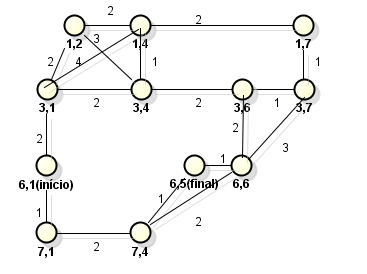
\includegraphics[keepaspectratio=true,scale=0.7]{figuras/grafohotspotcard2.PNG}
	\caption{grafo do exemplo 2 do \textit{hot-spot card} BestPath}
\end{figure}

Para o algorítimo A*, será gerado o grafo: 6,1 -> 7,1 -> 7,4 -> 6,6.

\section{EmbeddedCommunicator}

{\large \textbf{Nome do hot-spot:}} Embedded Communication

{\large \textbf{Graus de flexibilidade especificados:}}

\textbf{adaptação sem reinício:} não

\textbf{adaptação pelo usuário final:} não

{\large \textbf{Descrição geral}}

Implementa a comunicação via \textit{bluetooth} em hardwares diferentes, utilizando as bibliotecas disponíveis para cada kit.

\chapter{Código fonte}

O código fonte encontra-se disponível no seguinte endereço de repositório: 

https://github.com/rodrigorincon/path-planner-framework/tree/master/codigo/src 

Colaborando com a filosofia \textit{OpenSource}, o \textit{framework} pode ser utilizado por terceiros, sendo apenas requisitada a menção desse TCC como fonte inicial dos primeiros esforços.

Nesse caso, segue a referência ao TCC:

Rincon, Rodrigo Lopes. "Traveller: Um Framework de Definição de Trajetórias para Robôs Móveis". Trabalho de Conclusão de Curso. Universidade de Brasília (UnB), Faculdade do Gama (FGA), Curso de Engenharia de Software, Maurício Serrano (prof. orientador) e Milene Serrano (profa. coorientadora). Junho de 2014 a Julho de 2015.

\end{apendicesenv}
